\documentclass[usepdftitle=false]{beamer}
\usetheme{Berkeley}

% Packages
\usepackage{amsmath,amsfonts,amssymb} % ecuaciones
\usepackage{siunitx}
\usepackage{fancyhdr} % headers y footers
\usepackage{esint} % integrales cerradas
\usepackage{bbold} % para meter matriz identidad
\usepackage{graphicx} % estos dos para una figura
\usepackage{caption}
\usepackage{pdfpages} % para incluir declaracion IA
\usepackage{float}
\usepackage{url}
\usepackage[export]{adjustbox}
\usepackage[bottom]{footmisc}

\newcommand{\xd}{\dot{x}}
\newcommand{\xdd}{\ddot{x}}
\newcommand{\yd}{\dot{y}}
\newcommand{\ydd}{\ddot{y}}

\title[]{On wave propagation in solids and altermagnets}
\author{Victor Garcia Cervantes \\  [2\baselineskip] Supervisors: \\ Prof. Jasper van Wezel and Dr. Corentin Coulais}
\institute{University of Amsterdam}
\date{2025-2026}
\setbeamertemplate{footline}[frame number]

\begin{document}

\frame{\titlepage}

\begin{frame}{Contents}
\tableofcontents
\end{frame}

\section{Wave propagation}

\begin{frame}{Motivation}
    \begin{alertblock}{Idea}
        Guide wave signals in solids
    \end{alertblock}
    \pause 
    \vfill
    One can use different excitations: electrons, photons, phonons, etc.
    \pause
    \vfill
    \begin{enumerate}
        \item Unidirectional    \pause 
        \item Robust \pause $\longrightarrow$ topologically protected \pause 
        \item Spin-momentum locking
    \end{enumerate}
\end{frame}

\begin{frame}{Examples}
    Example 1: quantum spin Hall effect
    \begin{figure}
        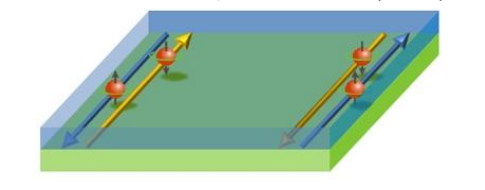
\includegraphics[width = 0.5\textwidth]{qshe_diagram.png}
    \end{figure} \pause 
    Example 2: 2D array of pendula
    \begin{figure}
        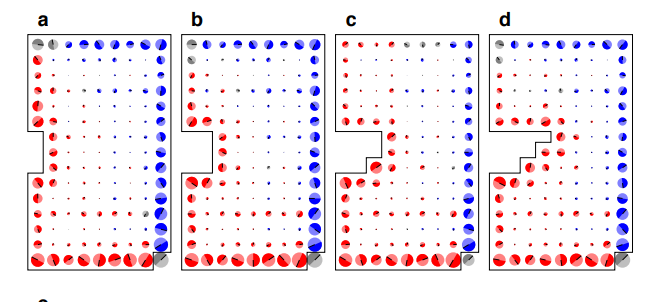
\includegraphics[width = 0.8\textwidth]{huber_pendula_diagram.png}
    \end{figure}
\end{frame}

\section{Altermagnets}

\begin{frame}[allowframebreaks]{What are altermagnets? A different phase of matter}
    \begin{figure}
        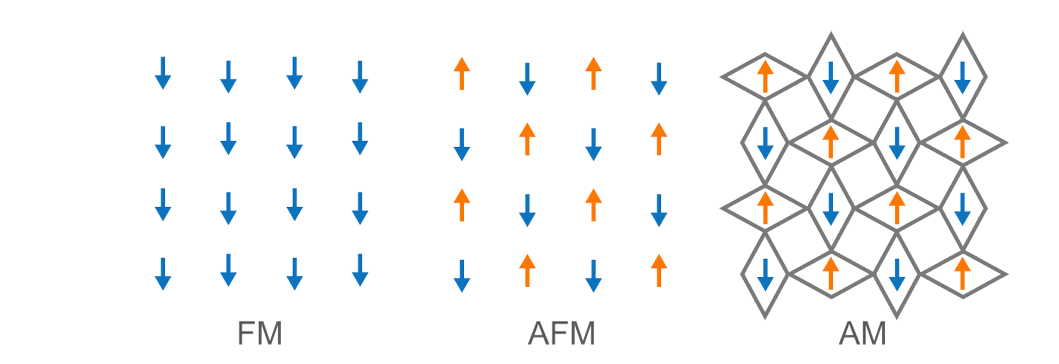
\includegraphics[width=\textwidth]{magnetism.png}
    \end{figure} 
    Kramer's theorem: TRS + half-integer spin $\Longrightarrow$ degenerate energies
    \framebreak
    \begin{enumerate}
        \item Symmetry: Rotation+TR denoted by $C_4\mathcal{T}$
        \item Zero magnetization  
        \item Spin-split bands
        \item $C_4\mathcal{T} \Longrightarrow N_\uparrow = N_\downarrow$
    \end{enumerate} 
    % include table comparing FM, AFM, AM
    \begin{figure}
        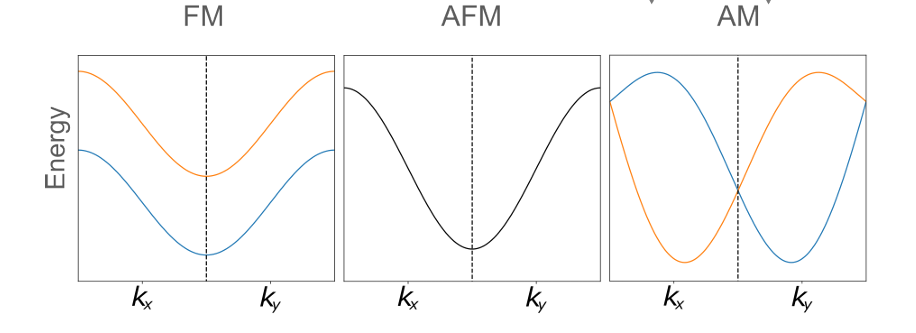
\includegraphics[width=\textwidth]{bands_altermagnet.png}
    \end{figure}
\end{frame}

\begin{frame}{Altermagnetic Lieb lattice}
    \pause
    \begin{figure}
        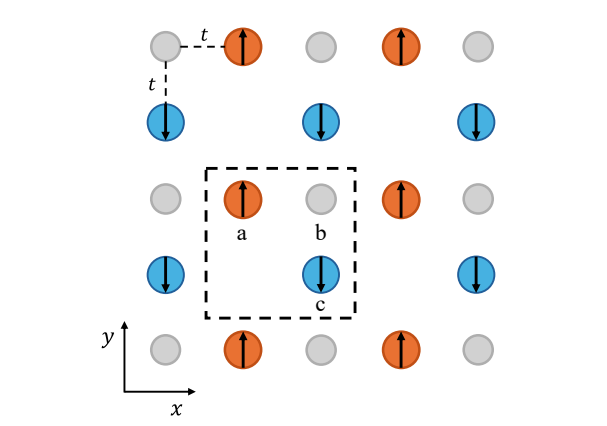
\includegraphics[width = 0.6\textwidth]{Lieb_lattice.png}
    \end{figure} \pause 
    It has hyperbolic bands:
    \begin{figure}
        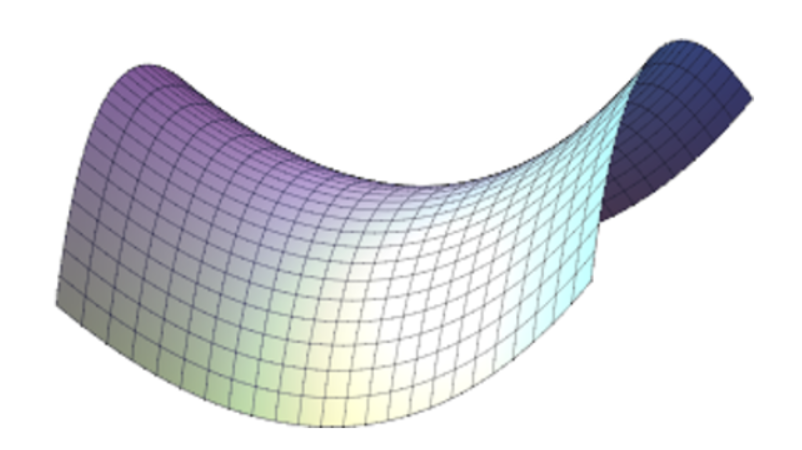
\includegraphics[width = 0.3\textwidth]{hyperbolic_paraboloid.png}
    \end{figure}
\end{frame}

\begin{frame}{Altermagnets have interesting properties}
    \begin{enumerate}
        \item Anisotropic wave propagation \vfill
        \begin{itemize}
            \item Unidirectional: control wave propagation direction  \vfill
            \item Spin-momentum locking: different spins propagate in different directions  \vfill
        \end{itemize}
        \item Piezomagnetism: magnetic moment is induced by strain 
        %\item Anomalous Hall effect 
    \end{enumerate}
    \vfill
    Useful in spintronics, spin-splitters, ultrafast photomagnetism, thermoelectrics ...
\end{frame}

\begin{frame}{Generalization of alter symmetry}
    \begin{alertblock}{Generalization alter symmetry}
        The spin can be substituted by any other 2-state variables.
    \end{alertblock}
    \vfill
    Some examples are:
    \begin{itemize}
        \item Photon polarization $\longrightarrow$ photonic altermagnet
        \item Electric dipole $\longrightarrow$ alterelectric
        \item Pendula chirality $\longrightarrow$ mechanical altermagnet (metamaterial)
    \end{itemize}
    \begin{figure}
        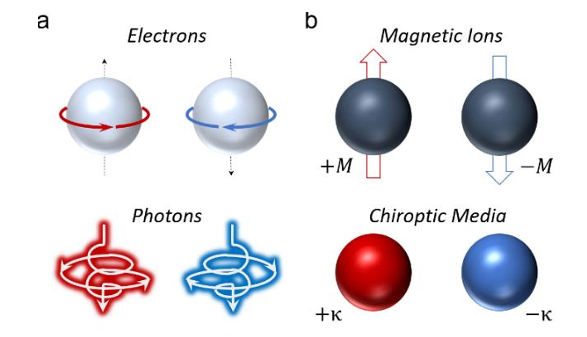
\includegraphics[width = 0.5\textwidth]{photonic_AM.png}
    \end{figure}
\end{frame}

\begin{frame}[allowframebreaks]{Metamaterials}
    Example 1: piezoelectricity
    \begin{itemize}
        \item Onsager relations: 
        \begin{align*}
        \varepsilon_{ij} &= S^E_{ijkl}\sigma_{kl} + d_{ijk}E_k, \\
        D_i &= d_{ijk}\sigma_{jk} + \kappa^\sigma_{ik}E_k,
        \end{align*}
        \item Restrictions due to crystal symmetry: 
        \begin{align*}
        \begin{bmatrix}
        d_{ij} \\
        \end{bmatrix}^T = 
        \begin{bmatrix}
        0 & 0 & 0 & d_{15} & 0 \\
        0 & 0 & 0 & d_{24} & 0 \\
        d_{31} & d_{32} & d_{33} & 0 & 0
        \end{bmatrix}^T \quad (j = 1, 2, 3, 4, 5, 6)
        \end{align*} 
        \item Enhancement due to complex structures  
        \item Properties given by its structure, not by its parts  
    \end{itemize}
    \framebreak
    Example 2: negative refractive index
    \begin{figure}
        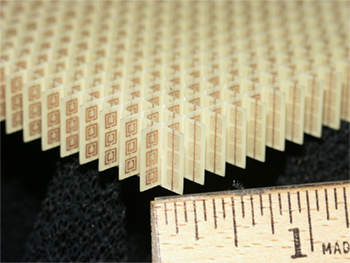
\includegraphics[width = 0.4\textwidth]{Split-ring_resonator_array_10K_sq_nm.jpg}
    \end{figure}
\end{frame}

\section{Non-hermiticity}

\begin{frame}{Non-hermiticity}
    \begin{itemize}
        \item Motivation: open systems \pause 
        \item Spectrum becomes complex
        \begin{figure}
        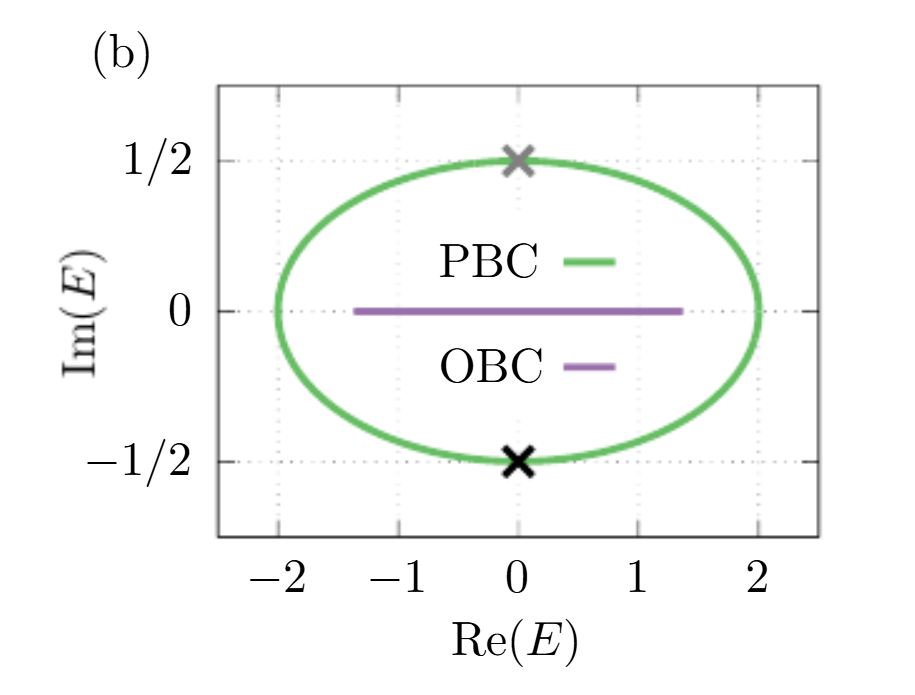
\includegraphics[width = 0.4\textwidth]{hatano-nelson_spectrum.png}
        \end{figure} \pause 
        \item Two major effects: bulk-boundary correspondence and non-hermitian skin effect \pause 
        \item Example: Hatano-Nelson model \pause 
        \begin{align*}
        \hat{H}_{\rm HN} = \sum_j \left[ t_Lc_{j+1}^{\dagger} c_j + t_Rc_j^{\dagger} c_{j+1} \right]
        \end{align*}
    \end{itemize}
\end{frame}

\begin{frame}{Non-reciprocity}
    \begin{minipage}[t]{0.65\textwidth}
        \begin{itemize}
            \item Motivation: classical analogue of non-hermiticity \pause
            \item Breaks inversion symmetry $\longrightarrow$ unidirectional waves \pause 
            \item Response differs when transmitter/receiver swapped \pause
            \item Breaks Newton's third law (classical level) \pause
            \item $\begin{pmatrix}
            F_1 \\ 
            F_2
            \end{pmatrix}
            =
            \begin{pmatrix}
            k & -k^o \\ 
            +k^o & k
            \end{pmatrix}
            \begin{pmatrix}
            \Delta_1 \\ 
            \Delta_2
            \end{pmatrix}$ \pause 
            \item Non-reciprocal units \pause 
            \item Leads to pendula chirality
        \end{itemize}
    \end{minipage}%
    \hfill
    \begin{minipage}[t]{0.3\textwidth}
        \vspace{0.5cm}
        \raggedleft
        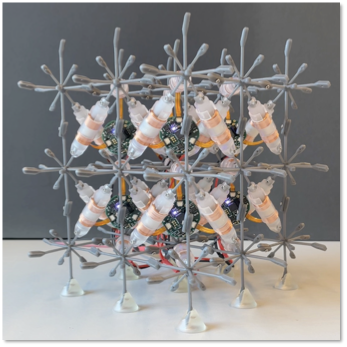
\includegraphics[width=\linewidth]{Yuan_cube_clear.png}
    \end{minipage}
\end{frame}

\section{Summary}

\begin{frame}{In practice}
    The procedure I have been following is:  
    \begin{enumerate}
        \item Choose a classical model  \pause 
        \item Write equations of motion  \pause 
        \item Multiple scale expansion \pause 
        \item Map to quantum system  \pause 
        \item Analyze spectrum and eigenstates \pause 
    \end{enumerate}
    \vfill
    The idea is to apply them to increasingly more complex models.
    \vfill
    Experimentally: build a Lieb lattice of non-reciprocal pendula and compare with theoretical predictions
\end{frame}

\begin{frame}{Summary}
    \begin{alertblock}{Goal}
        Study altermagnetism and non-hermiticity in classical analogues 
    \end{alertblock}
    \vfill
    \begin{itemize}
        \item Altermagnets: $C_4\mathcal{T}$ symmetry can lead to unidirectional and spin-momentum locking propagation \vfill
        \item Non-hermitian skin effect: waves localized at boundaries \vfill
        \item Classical analogues enable experimental realization
    \end{itemize}
\end{frame}

\begin{frame}{References}
    \footnotesize
\begin{thebibliography}{99}
\bibitem{visser} Visser, A. \textit{Master Thesis}. University of Amsterdam (2025).
\bibitem{huber} Huber, S. D. \textit{Nat. Phys.} \textbf{12}, 621 (2016).
\bibitem{smejkal} Smejkal, L. et al. \textit{Phys. Rev. X} \textbf{12}, 040501 (2022).
\bibitem{gao} Gao, Y. et al. \textit{Mater. Today} \textbf{48}, 25 (2021).
\bibitem{sato} Sato, M. et al. \textit{Phys. Rep.} \textbf{910}, 1 (2021).
\end{thebibliography}
\end{frame}

% Annex slides remain the same...
\section*{Annex}

\begin{frame}[noframenumbering]{Activity}
    The classical analogue of non-hermiticity of Hatano-Nelson is non-reciprocity. \pause
    \vfill
    Activity: internal energy source. \pause 
    \vfill
    There are different ways to achieve activity:  \pause
    \begin{itemize}
        \item Negative damping \pause
        \item Time delay \pause 
        \item \textbf{Non-reciprocity}
    \end{itemize}
\end{frame}

% ... rest of annex frames ...

\end{document}